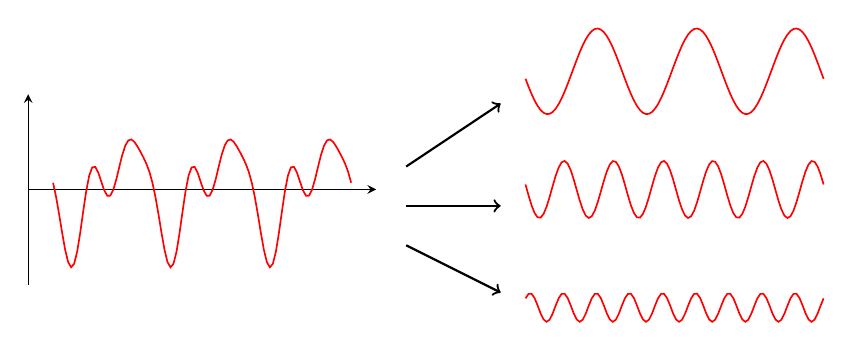
\begin{tikzpicture}
\begin{axis}[
    width=6cm, 
    height=4cm,
    axis x line=center, 
    axis y line=middle, 
    samples=100,
    ymin=-2, ymax=2,
    xmin=0, xmax=11,
    domain=0.25*pi:3.25*pi,
    ticks=none
]
\addplot [mark=none, semithick, red] {0.9*cos(2*deg(x)+10)-0.6*cos(4*deg(x)+80)+0.3*cos(6*deg(x)+40)};
\end{axis}
\begin{axis}[at={(6cm,1.5cm)},hide axis,
    width=6cm, 
    height=4cm,
    samples=100,
    ymin=-2, ymax=2,
    xmin=0, xmax=11,
    domain=0.25*pi:3.25*pi,
    ticks=none
]
\addplot [mark=none, semithick, red] {0.9*cos(2*deg(x)+10)};
\end{axis}
\begin{axis}[at={(6cm,0cm)},hide axis,
    width=6cm, 
    height=4cm,
    samples=100,
    ymin=-2, ymax=2,
    xmin=0, xmax=11,
    domain=0.25*pi:3.25*pi,
    ticks=none
]
\addplot [mark=none, semithick, red] {-0.6*cos(4*deg(x)+80)};
\end{axis}
\begin{axis}[at={(6cm,-1.5cm)},hide axis,
    width=6cm, 
    height=4cm,
    samples=100,
    ymin=-2, ymax=2,
    xmin=0, xmax=11,
    domain=0.25*pi:3.25*pi,
    ticks=none
]
\addplot [mark=none, semithick, red] {0.3*cos(6*deg(x)+40)};
\end{axis}
\draw[->, thick] (4.8, 1.5)--(6, 2.3);
\draw[->, thick] (4.8, 1.0)--(6, 1.0);
\draw[->, thick] (4.8, 0.5)--(6, -0.1);
\end{tikzpicture}
